In diesem Abschnitt soll auf die Datenaufnahme sowie alle nötigen Schritte der Datenverarbeitung bis zur fertigen $g^{(2)}(\tau)$-Funktion eingegangen werden. 
Dafür werden zuerst die Datenaufnahme und dafür nötige Kalibrationsverfahren erläutert. 
In diesem Zuge wird zudem auf das Aussehen der aufgenommenen Daten (Waveforms) eingegangen. 
Anschließend werden korrelierte Einzeldateien betrachtet und es wird verdeutlicht, warum eine Mittelung vieler Waveforms unumgäglich ist. 
Zuletzt werden angewandte Korrekturen und Filter angesprochen sowie verdeutlicht, wie die Mittelung der Daten erfolgt. 

\subsection{Datenaufnahme und Waveforms}
\label{ssec:Datenaufnahme und Waveforms}
Die Aufnahme der Daten erfolgt durch ein von der Arbeitsgruppe geschriebenes Programm, welches mit den ADCs kommuniziert. Ein Screenshot der GUI, auf dem die wichtigsten Schritte der Datenaufnahme markiert sind, ist in \autoref{fig:Screenshot GUI} eingefügt. 
\begin{figure}[h]
    \centering
    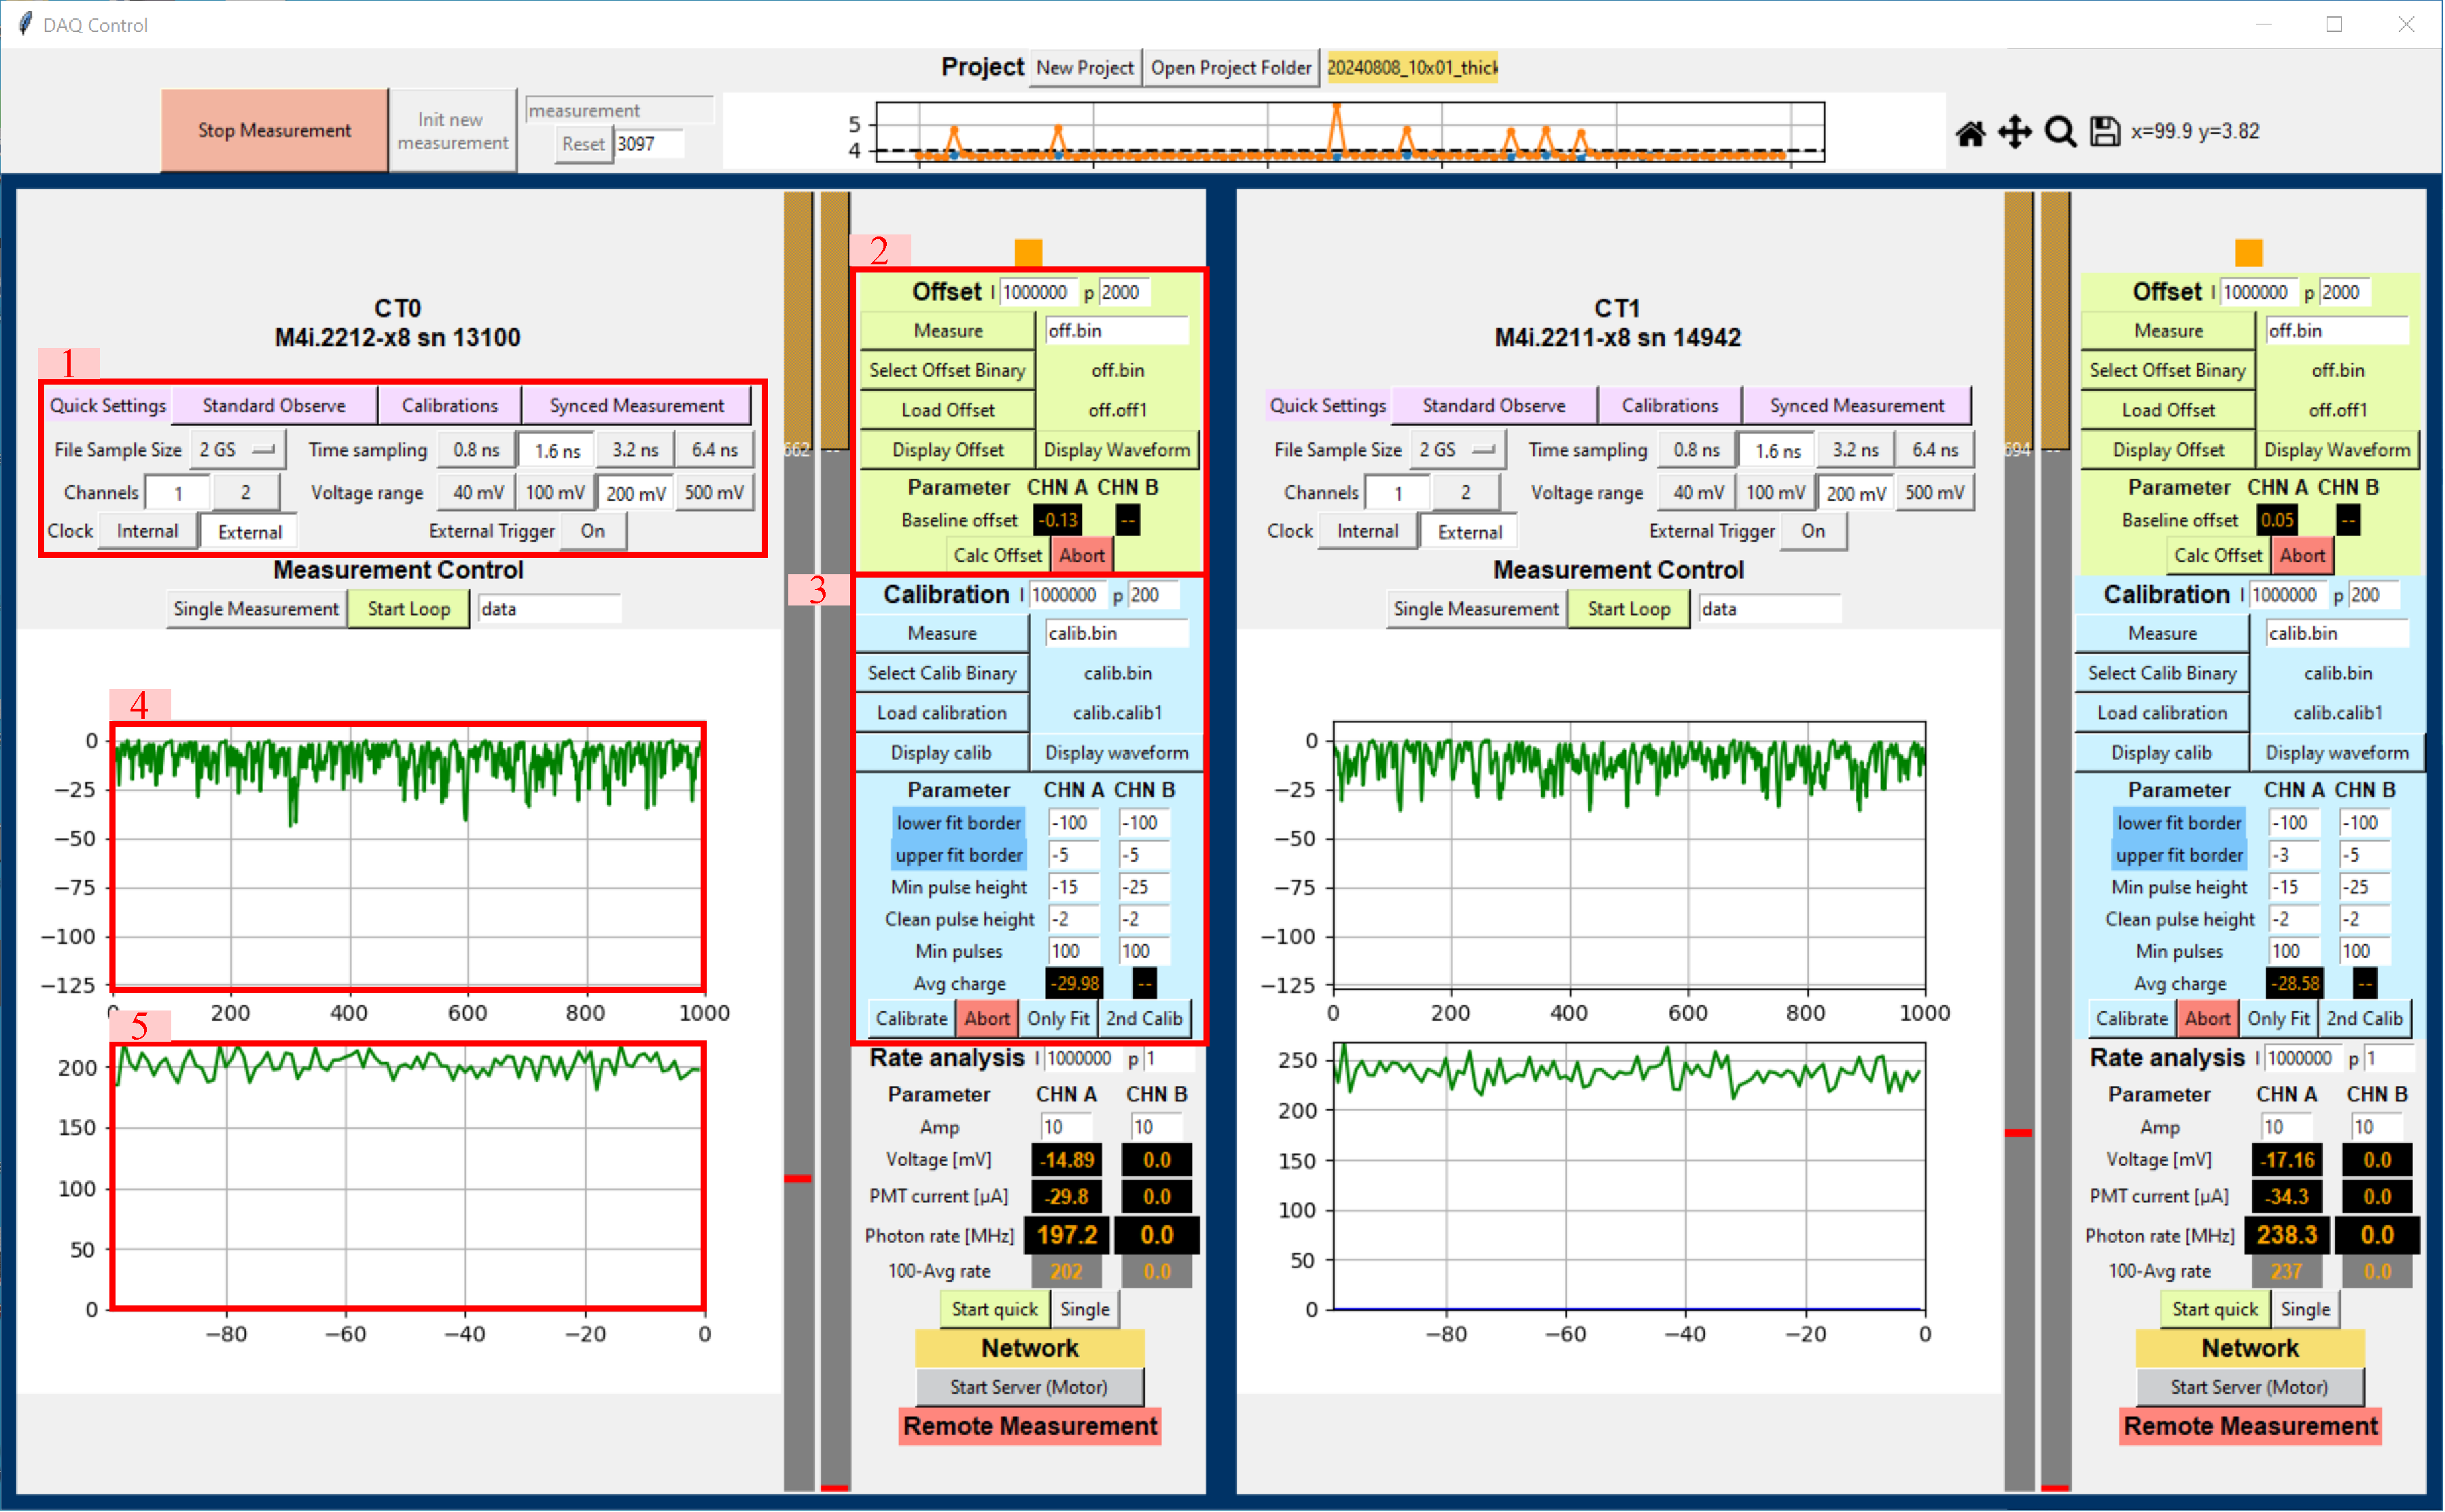
\includegraphics[width=0.9\textwidth]{images/Datenaufnahme/GUI.pdf}
    \caption{Dargestellt ist ein Screenshot der GUI zur Datenaufnahme. Wichtige Schritte sind markiert.}
    \label{fig:Screenshot GUI}
\end{figure}
In der GUI wird für jede verwendete Digitalisierungskarte ein Fenster erstellt, in dem Einstellungen für die jeweilige Karte vorgenommen werden können. 
Nach dem Erstellen eines Projekts können in dem mit \emph{1} markierten Bereich in \autoref{fig:Screenshot GUI} Einstellungen für die ADC-Karte vorgenommen werden. 
Es wird mit einem Kanal je Karte gemessen und die Samplingzeit beträgt $1{,}6$\,ns bei einer Dateigröße von 2 Gigasamplen. 
Der zu digitalisierende Spannungsbereich wird passend zu den in \emph{4} abgebildeten Waveforms auf 200\,mV gesetzt. 
Clock und Trigger werden extern durch das White Rabbit System gegeben. 
Die genannten Einstellung werden größtenteils vor der Messung automatisch mit dem Button \glqq Init new measurement\grqq\;gesetzt. \\
Vor Start der Messung müssen zwei Kalibrationsschritte für jeden Kanal gemacht werden. 
Zuerst wird unter \emph{2} eine Offset-Kalibration durchgeführt, indem \glqq Measure\grqq\;und \glqq Calc Offset\grqq\;gewählt werden. 
Diese wird ohne Beleuchtung und mit ausgeschalteter Hochspannung durchgeführt. 
Das Programm bestimmt diesen vom PMT abhängigen Offset und entfernt diesen, sodass dieser die Korrelation nicht beeinflusst \cite{zmijaOpticalIntensityInterferometry2021}. 
Anschließend wird bei eingeschalteter Hochspannung und niedriger Photonenrate eine Raten-Kalibration durchgeführt, sodass gemessene Spannungen in Photonenraten umgerechnet werden können. 
Dies ist nötig, da aufgrund der hohen Raten bei der Messung nicht Einzelphotonepulse, sondern ganze Waveforms miteinander korreliert werden. 
Für die Kalibration wird für jeden Kanal die mittlere Pulsform der PMT-Pulse bestimmt und gespeichert. 
Es wird erwartet, dass diese einen bedeutenden Einfluss auf die Form der $g^{(2)}$-Funktion hat, da die Photonenpulse deutlich breiter sind als die einzelnen $1{,}6$\,ns-Bins, was zu einer Korrelation benachbarter Bins führt \cite{zmijaOpticalIntensityInterferometry2021}. 
Aus den gemessenen Daten wird bestimmt, wie viel Ladung ein Photon, das auf einen PMT trifft, durchschnittlich freisetzt, woraus anschließend die in \emph{5} gezeigten Photonenraten in MHz bestimmt werden können. \\
Nach diesen Kalibrationsschritten kann die Messung gestartet werden, woraufhin synchronisiert durch den Trigger des White Rabbit Systems 2$\cross$2\,GS Daten aufgenommen werden. 
Dies entspricht einer Messdauer von $3{,}436\,\mathrm{s}$. 
Nach Ablauf von 4\,s startet anschließend der nächste Trigger eine Messung von 2$\cross$2\,GS, sodass idealerweise ein Duty-Cycle von 85{,}9\% erreicht wird \cite{zmijaFirstIntensityInterferometry2023}. 
Da jedes Sample einem 8\,bit ADC-Wert entspricht, erreicht die Messung also eine Datenrate von 2$\cross$2\,GB alle 4\,s, was erklärt, weshalb die Daten erst gespeichert und anschließend offline korreliert werden. 
Zur Veranschaulichung ist in \autoref{fig:Offest_Rate Kalibration} aufgezeigt, wie eine typische Waveform zur Offset- bzw. Raten-Kalibration und zur Messung aussieht. 
\begin{figure}[h]
    \centering
    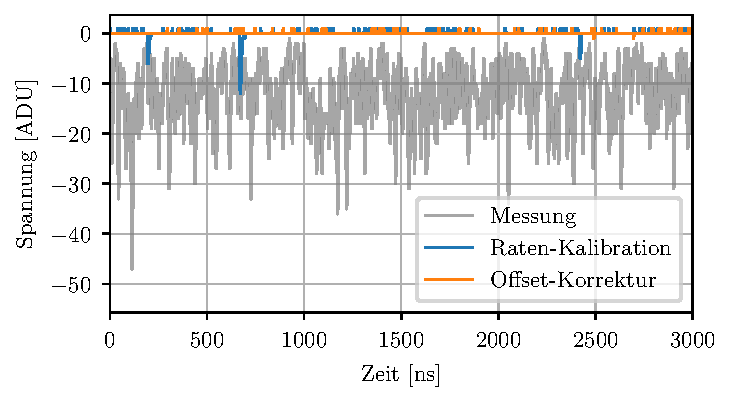
\includegraphics{images/Datenaufnahme/Kalibration.pdf}
    \caption{Abgebildet ist der Ausschnitt einer Waveform für die Offset Kalibration (ausgeschaltete Hochspannung und Beleuchtung), Raten-Kalibration (Hochspannung und Licht an, niedrige Photonenrate) und für die Messung.}
    \label{fig:Offest_Rate Kalibration}
\end{figure}

\subsection{Korrelation}
\label{ssec:Korrelation}
Die Korrelation der Daten erfolgt parallelisiert, nachdem die Datenaufnahme abgeschlossen ist. 
Jede Datei von beiden Kanälen wird getrennt miteinander korreliert, indem diese zuerst in Vektoren $\mathbf{A}$ und $\mathbf{B}$ eingelesen werden. 
Anschließend wird für jede Zeitdifferenz $\tau$ das folgende Skalarprodukt berechnet: 
\begin{equation}
    G^{(2)}(\tau) = \mathbf{A}(t)\cdot\mathbf{B}(t+\tau)
    \label{eq:korrelation}
\end{equation}
Damit entspricht jeder Wert von $G^{(2)}(\tau)$ der unnormierten zeitlichen Photonenkorrelation zu diesem Zeitpunkt \cite{zmijaOpticalIntensityInterferometry2021}. 
Die korrelierten Einzeldateien können anschließend für die weitere Datenanalyse gespeichert werden, da diese deutlich kleiner (im Bereich weniger kB) sind als die Rohdaten. 
Um aus einer bestimmten $G^{(2)}$-Funktion die normierte zeitliche Korrelationsfunktion zu erhalten, wird diese durch ihren Mittelwert weit außerhalb des Bunching Peaks geteilt:
\begin{equation}
    g^{(2)}(\tau) = \frac{G^{(2)}(\tau)}{\overline{G^{(2)}(\tau\gg\tau_c)}}
    \label{eq:G2 normalisierung}
\end{equation}
Ein Beispiel für die unnormierte Funktion $G^{(2)}$ einer einzelnen Datei ist in \autoref{fig:G2(tau)} dargestellt. 
\begin{figure}[h]
    \centering
    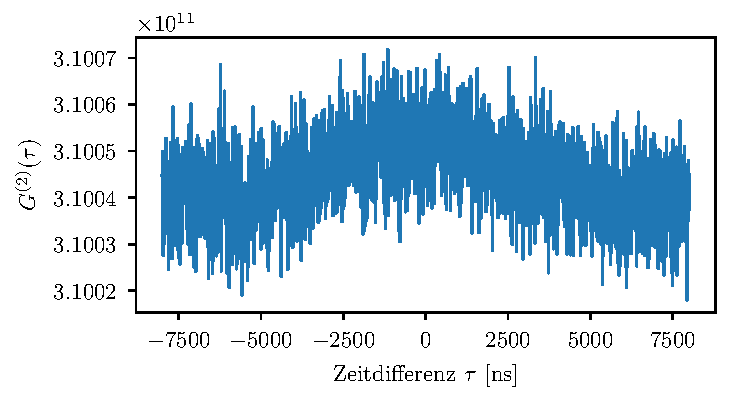
\includegraphics{images/Datenaufnahme/G2.pdf}
    \caption{Ein Beispiel einer unnormierten Korrelationsfunktion ist abgebildet. Durch das verrauschte Signal ist an der Stelle $\tau=0$ kein Bunching Peak sichtbar.}
    \label{fig:G2(tau)}
\end{figure}
Es ist ersichtlich, dass die Funktion stark verrauscht ist und der Bunching Peak nicht auszumachen ist. 
Die in \autoref{ssec:Intensitäteninterferometrie} bereits erwähnte Nowendigkeit der Mittelung über viele Daten, d. h. lange Zeiten, um die Form von $g^{(2)}$ bestimmen zu können, ist daher deutlich sichtbar. 

\subsection{Mittelung der Daten und Filter}
\label{ssec:mittelung und filter}
Wie bereits im vorangegangenen Abschnitt ersichtlich wurde, ist eine Mittelung vieler Dateien unumgänglich, um den Bunching Peak analysieren zu können. 
Hierbei wird der Ansatz eines gewichteten Mittelwerts gewählt, da nicht jede der etwa $3{,}4\,\mathrm{s}$ langen Dateien statistisch gleich aussagekräftig ist. 
So weisen manche der Messabschnitte höhere Photonenraten auf als andere (vgl. dazu \autoref{fig:Screenshot GUI}, Kasten \emph{5}). 
Unter der Annahme, dass ein Großteil des Rauschens in der $G^{(2)}$-Funktion statistischen Fluktuationen entspricht, wird erwartet, dass das Rauschen für höhere Photonenraten abnimmt. 
Dies bedeutet, dass Dateien mit höheren Raten und geringerer Schwankung stärker gewichtet werden sollten, als jede mit geringeren Photonenraten. 
Um dies zu bewerkstelligen, wird von jeder Datei $G^{(2)}_i$ die Standardabweichung $\sigma_i$ bestimmt und anschließend der folgende gewichtete Mittelwert berechnet \cite{cochranProblemsArisingAnalysis1937}:
\begin{equation}
    \overline{G^{(2)}} = \frac{\sum_{i=0}^{n}\frac{G^{(2)}_i}{\sigma_i^2}}{\sum_{i=0}^{n} \sigma_i^{-2}}
\end{equation}
Das Ergebnis der Mittelung über 10000 Dateien, d. h. etwa $9{,}5$\,h Korrelationsdaten, ist in \autoref{fig:gemittelte G2 vs g2} oben abgebildet. 
Der Bunching Peak bei $\tau\approx 0$ ist nach Mittelung der Daten bereits sichtbar. 
Allerdings sind durch die Mittelung weitere Artefakte ersichtlich geworden. 
Bereits in den korrelierten Einzeldateien ist eine Struktur in den Daten zu erkennen, welche das Signal überlagert. 
Nach der Mittelung ist diese nun besonders deutlich, was darauf hinweist, dass sie nicht von rein statistischer Natur ist, sondern tatsächlich zwischen den Kanälen korreliert ist. 
Das etwa $12\,\mathrm{\mu s}$ breite Störsignal kommt von der Spannungsversorgung der Xenonlampe \cite{zmijaOpticalIntensityInterferometry2021}, liegt daher in beiden Kanälen zugleich vor und wird deshalb durch die Korrelation und Mittelung verstärkt. 
Da es aber mehrere Größenordnungen breiter ist als der Bunching Peak und diesen daher kaum beeinflusst, wird es in diesem Abschnitt erst einmal vernachlässigt. 
In einem späteren Abschnitt zur Integration des Peaks wird auf eine Methode eingegangen, dieses Störsignal zu entfernen. \\
\begin{figure}[h]
    \centering
    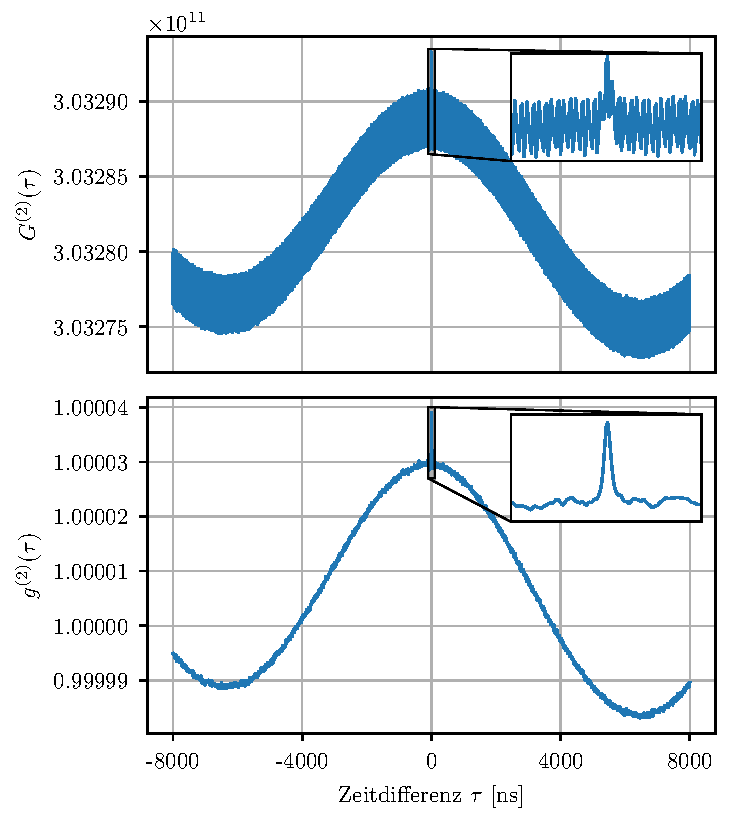
\includegraphics{images/Datenaufnahme/G2_vs_g2.pdf}
    \caption{Dargestellt sind der Unterschied zwischen $G^{(2)}(\tau)$ und der normierten Funktion $g^{(2)}(\tau)$ nach Mittelung über 10000 Dateien, bei der zudem die \glqq pattern correction\grqq\;und der Tiefpass angewandt worden sind. Es ist deutlich erkennbar, dass die angewandten Methoden zu einer starken Verbesserung des Signal-Rausch-Verhältnisses geführt haben. }
    \label{fig:gemittelte G2 vs g2}
\end{figure}

Weiterhin ist durch Zoom in die Daten oder eine Fouriertransformation dieser ein 8-Bin-periodisches Muster zu erkennen, welches dafür verantwortlich ist, dass die $G^{(2)}$-Funktion ein breites Band an Werten annimmt. 
Dieses von den ADC-Karten kommende Muster stört den Verlauf des Bunching Peaks zudem in beträchtlicher Weise, da es sich auf der selben Zeitskala wie der Peak selbst befindet. 
Da das Störsignal von den beiden ADC-Karten gleichzeitig ausgeht, ist dieses korreliert und daher besonders dominant in der abgebildeten $G^{(2)}$-Funktion.
Um das Störsignal zu entfernen, wird eine von der Arbeitsgruppe geschriebene \glqq pattern correction\grqq\;angewandt, welche in den ersten 4000 Bins (d. h. im Intervall $\tau\in[-8000,-1600]\,\mathrm{ns}$) jeweils 8 Bins mittelt und die Daten anschließend durch das so ermittelte Muster teilt. 
Da das Muster sowohl das eigentliche 8-Bin-periodische Muster, als auch den Offset der $G^{(2)}$-Funktion, wie er in \autoref{eq:G2 normalisierung} definiert ist, enthält, wird diese durch die Division automatisch auch normiert. 
Der Schritt der \glqq pattern correction\grqq\;wird für jede Datei separat vor der Bildung des Mittelwertes angewandt. \\
Nach diesen Schritten wird auf die gemittelte $g^{(2)}$-Funktion noch ein digitaler Tiefpass 2. Ordnung mit einer Grenzfrequenz von 200\,MHz angewandt, um weitere hochfrequente Störsignale zu entfernen. 
Die nach erwähnten Korrekturen und der angewandten Mittelung erhaltene Funktion $g^{(2)}(\tau)$ ist in \autoref{fig:gemittelte G2 vs g2} unten abgebildet. 

